\chapter{Data Analysis}
\label{ch:data-analysis}

The initial goal of this project was concerned with modeling different infection patterns as influenced through \gls{sirna} mediated gene knockdown. By fitting a \gls{glm} model, using the large set of available cellular features, described in section \ref{sec:scf-data}, as predictor variables and the membership to one of two wells as binary response, it was conjectured that it is possible to determine a subset of most influential features. Unfortunately, to present date, this could not be executed in a sensible manner.

In order the make the substantial amount of single cell data, obtained from several large-scale, high throughput \gls{sirna} screens performed by the InfectX consortium, available to an environment for statistical analysis, an R packages was developed, which is described in chapter \ref{ch:singlecellfeatures}. Building on this crucial piece of infrastructure, the current chapter will explore some of the data analysis that was performed, beginning a short introduction into the theory of \glspl{glm} and continuing with preliminary findings that motivate the investigation of desirable normalization schemes. A final outlook on potential improvements will conclude this chapter.

\section{Statistical Models}
Many algorithms for binary classification exist, including decision trees, \glspl{svm}, Bayesian networks, neural networks and \glspl{glm}, some of which have been encountered in previous sections due to their application in infection scoring (see section \ref{sec:infection-scoring}). As neither prediction not classification per se are of main interest, binary logistic regression presents an attractive method due to availability of extensive coefficient and model statistics. Therefore, modeling of \gls{sirna} effects on cellular features is performed, using the glm function provided by the R stats package \citep{RCoreTeam2015}, as well as glmnet belonging to the CRAN package of the same name \citep{Friedman2010a}.

A large number of binary comparisons are possible with the given datasets. In order to focus on attractive wells in the sense that there is reason to assume they might be biologically interesting, the $n \choose 2$ possible combinations of wells (within a single plate, \tilde 70000 pairs can be formed), are narrowed down using a \gls{pmm} as derived by \cite{Ramo2014}. Of the resulting hit list, several genes are selected and compared to wells containing scrambled \gls{sirna} reagents, which should provide a good choice for establishing a background behavior. A possible control alternative are mock wells but owing to the complete absence of \gls{sirna} molecules, the difference in treatment of cells is only increased and hence it can be argued that they provide inferior comparisons.

\subsection{Generalized Linear Models}
Modeling the relationship among variables is one of the most important applications of statistical theory. The study of regression analysis (and the closely related notion of correlation) started to form towards the end of the 19th century with Sir Francis Galton's study of height heredity in humans and his observation of regression towards the mean. Over the next few years, Udny Yule and Karl Pearson cast the developed concepts into precise mathematical formulation, in turn building on work performed by Adrien-Marie Legendre and Carl Friedrich Gauss who developed the method of least squares almost a century earlier \citep{Allen1997}.

A multiple linear regression model can be written in matrix-vector form as
\begin{equation}
  y = X \beta + \epsilon \label{eq:lin-reg}
\end{equation}
where $y \in \R^n$ is the vector of observations on the dependent variable, the design matrix $X \in \R^{n \times p}$ contains data on the independent variables, $\beta \in \R^p$ is the $p$-dimensional parameter vector and the error term $\epsilon \in \R^n$ captures effects not modeled by the regressors.

In order to find unknown coefficients $\beta_i$, the ordinary least squares estimator minimizes the residual sum of squares, the squared differences between observed responses and their predictions according to the linear model.
\begin{subequations}
\begin{align}
  \Hbeta &= \argmin_{\beta} \norm{y - X \beta}^2 \\
         &= (X^T X)^{-1} X^T y \label{eq:ols-estimate}
\end{align}
\end{subequations}
Some assumptions are typically associated with linear regression models that yield desirable attributes for the estimates. None of these restrictions are imposed on the explanatory variables; they can be continuous or discrete and combined as well as transformed arbitrarily. Furthermore, in practice, it is irrelevant whether the covariates are treated as random variables or as deterministic constants. With exception of the field of econometrics it appears that the majority of literature adheres to the latter interpretation and therefore, statements will not explicitly be conditional on covariate values.
\begin{description}
  \item[Linearity.] The relationship between dependent and independent variables is assumed to be linear (after suitable transformations) and individual effects additive. If this cannot be satisfied, a linear model is not suitable.
  \item[Full rank.] For the matrix $X^T X$ to be invertible, it has to have full column rank $p$. Therefore $n \geq p$ and all covariates must be linearly independent.
  \item[Exogeneity.] All independent variables should be known exactly i.e. contain no measurement or observation errors as only the mean squared error of the dependent variable is minimized. Additionally, all important causal factors have to be included in the model. Exogeneity implies $\Erw[\epsilon_i] = 0 \forall i$, as well no correlation between regressors and error terms \citep{Hayashi2000}.
  \item[Spherical errors.] This includes both homoscedasticity or constant error variance, $\Erw[\epsilon_i^2] = \sigma^2 \forall i$, and uncorrelated errors $\Erw[\epsilon_i \epsilon_j] = 0 \forall i \neq j$. These two conditions can be written more compactly as $\Var(\epsilon) = \sigma^2I_{n \times n}$.
  \item[Normality.] For the estimated coefficients to gain some additional desirable characteristics, it can be required that the errors $\epsilon_i$ be jointly normally distributed. Together with the above restrictions on expectation and variance, this yields $\epsilon \mathbin{\sim} \N_n(0, \sigma^2 I_{n \times n})$.
\end{description}

Violations of these assumptions have varying consequences. In situations of perfect collinearity, the ordinary least squares estimator $\Hbeta$ as defined in \eqref{eq:ols-estimate} does not exist. Recovering such a situation is possible by using a generalized matrix inverse (for example the Moore--Penrose pseudoinverse) or by dropping the corresponding variables. High correlation inflates coefficient variances, which may be countered by employing a regularization scheme like ridge regression. Omitting a variable that is both correlated with dependent variables and has an effect on the response (a nonzero true coefficient) will introduce bias in the parameters. The method of instrumental variables can help to produce an unbiased estimator nonetheless.

The assumption of spherical errors ensures that the least squares estimator is the best linear unbiased estimator in the sense that it has minimal variance among all linear unbiased estimators. Heteroscedasticity and autocorrelation do not yield biased coefficient estimates but can introduce bias in \gls{ols} estimates of variance, causing inaccurate standard errors. Such a situation calls for generalized least squares estimation, for example weighted least squares when the data is not homoscedastic ($\sigma^2$ is vector-valued but off-diagonal elements of $\Var(\epsilon)$ are zero), or feasible generalized least squares which can be applied in case of heteroscedasticity and\slash or correlation between errors. Whenever the condition of spherical errors does not hold, \gls{ols} is inefficient and generalized least squares estimators have smaller variance.

Finally, normality provides the framework necessary for applying common hypothesis testing, yielding t-statistics, p-values and confidence intervals for coefficients, as well as an F-statistic for the model as a whole. Furthermore, under normality assumptions, the \gls{ols} estimator and \gls{mle} coincide. Quantile regression and other forms of robust regression, such as M estimators may restore validity of inference when errors do not follow a normal distribution.

Modeling data to a dichotomous response variable with \gls{ols} methodology, while readily possible, often is a bad choice due to violations of several of the above assumptions. First of all, normal distributions are continous with support $x \in \R$ and thusly a categorical variable cannot be normally distributed. Homoscedasticity does not hold either, as can easily be seen in a geometric argument: any line with nonzero slope, fitted to a set of $Y$ with $Y_i \in \{0,1\}$, will produce residuals that vary linearly. Finally and perhaps most importantly, a linear model is unsuitable due to there being no constraints on the range of fitted values. While this by itself could be dealt with, the concept of additivity within this context raises questions of its own when fitted values are thought of as probabilities. Linear behavior throughout the range of 0 (impossible) to 1 (certain) makes little sense for most practical applications, as typically, some flattening is expected when approaching either end of the spectrum.

In view of the above considerations it becomes clear that some sort of extension to ordinary linear regression in needed in order to deal with binary response variables. A theory, unifying several previously separately treated statistical models, including linear regression, \gls{anova}, logistic regression, Poisson regression and multinomial response, as \acrfullpl{glm}, was developped by John Nelder and Robert Wedderburn in the early 1970's \citep{Nelder1972}. Much of this section is based on that work.

In order to accommodate the newly added extensions, the classical linear model is rewritten as

\begin{equation}
  \Erw[Y] = \mu \text{ where } \mu = X \beta,
\end{equation}

yielding a three-part specification, consisting of

\begin{enumerate}[label=(\alph*)]
  \item the \textit{random component}; $Y$ is distributed according to a member of the exponential family,\footnote{Many of the predominately used distributions belong to the exponential family, including but not restricted to Bernoulli, binomial, Poisson, exponential and normal distributions. Common to all members, the probability density function can be written as
  \begin{equation}
    f(x;\theta) = h(x) e^{\theta^\intercal T(x)-A(\theta)}
  \end{equation}
  where $\theta$ is the vector of paramteters, $T(x)$ the vector of sufficient statistics, $A(\theta)$ the cumulant generating function and $h(x)$ the base measure. In case of the Bernoulli distribution
  \begin{equation}
    f(k;\pi) = \pi^k (1-\pi)^{1-k}\label{eq:bern-pmf}
  \end{equation}
  this gives $h(k) = 1$ $T(k) = k$, $\theta = \log\frac{\pi}{1-\pi}$ and $A(\theta) = \log(1+e^\theta)$. Restricting \glspl{glm} to exponential family distributions makes it possible to stay within the framework of maximum likelihood parameter estimations, as given this restriction, \gls{mle} yields the best parameter estimator with respect to minimal variance.}
  \item the \textit{systematic component}; a linear predictor is given by $\eta = X\beta$,
  \item and the \textit{link} between random and systematic components, expressed as the link function $g(\cdot)$, such that $\eta = g(\mu)$; in case of normally distributed Y, $\mu = \eta$ (identity link).
\end{enumerate}

\renewcommand{\arraystretch}{2}
\setlength{\tabcolsep}{0.2em}
\begin{table}
  \centering
  \caption[Link functions of common univariate distributions of the exponential family.]{Common univariate distributions of the exponential family alongside mean and canonical link functions.}
  \label{tab:glm-links}
  \footnotesize
  \begin{tabular}{L{0.18\linewidth}L{0.18\linewidth}L{0.18\linewidth}L{0.18\linewidth}L{0.18\linewidth}}
    Distribution &
      Support &
      Link name &
      Link function &
      Mean function \\
    \hline 
    Normal &
      $(-\infty, +\infty)$ &
      identity &
      $\eta = \mu$ &
      $\mu = X\beta$\\
    Poisson &
      $\{0, 1, 2, \dotsc\}$ &
      log &
      $\eta = \log(\mu)$ &
      $\mu = e^{X\beta}$\\
    Binomial &
      $\{0, 1, \dotsc, N\}$ &
      logit &
      $\eta = \log\left(\frac{\mu}{1-\mu}\right)$ &
      $\mu = \frac{e^{X\beta}}{1+e^{X\beta}}$\\
    Gamma &
      $(0, +\infty)$ &
      reciprocal &
      $\eta = -\mu^{-1}$ &
      $\mu = -(X\beta)^{-1}$\\
    Inverse Gaussian &
      $(0, +\infty)$ &
      inverse squared &
      $\eta = -\mu^{-2}$ &
      $\mu = (-2X\beta)^{-1/2}$\\
  \end{tabular}
\end{table}

Mean and canonical link functions for several common univariate distributions belonging to the exponential family are shown in table \ref{tab:glm-links}. Binary response can be written as 
\begin{equation}
  Y_i \mathbin{\sim} \Bern(\pi_i)
\end{equation}
which implies that
\begin{equation}
  \P(Y_i=1) = 1 - \P(Y_i=0) = \pi_i.
\end{equation}
Therefore, $\pi_i$ can be thought of as the probability of one outcome (i.e. success) and its complement ($1-\pi_i$) corresponds to the probability of the other outcome (failure). Each experimental unit that yields one outcome is associated with a vector of independent variables $x_i = (x_{i,1}, x_{i,2}, \dotsc, x_{i,p})$ and the goal of regression in this context becomes modeling the relationship between response probability $\pi_i$ and explanatory variables $x_{i}$. A suitable link function for Bernoulli distributed response, as discussed above, is required to map the unit interval onto the whole real line and preferably be shaped sigmoidally in order accurately describe increasingly likely as well as increasingly unlikely events. Three possibilities are often considered within this context,

\begin{enumerate}[label=(\alph*)]
  \item the \textit{logit} or logistic function
  \begin{equation}
    g(\pi) = \log\left(\frac{\pi}{1-\pi}\right),
  \end{equation}
  \item the \textit{probit} or inverse normal function
  \begin{equation}
    g(\pi) = \Phi^{-1}(\pi),
  \end{equation}
  with $\Phi(\cdot)$ denoting the cumulative distribution function of the normal distribution,
  \item and the \textit{complementary log-log} function
  \begin{equation}
    g(\pi) = \log\left(-\log(1-\pi)\right).
  \end{equation}
\end{enumerate}

All three functions are continuous and increasing on $(0,1)$ and the first two are symmetric in the sense that $g(\pi) = -g(1-\pi)$, while the third is not. Using a logit link function, the probability of a positive response can therefore be written as
\begin{equation}
  \pi_i = \frac{e^{x_i^\intercal \beta}}{1+e^{x_i^\intercal \beta}}
\end{equation}
and the model is, slightly rearranged, stated as
\begin{equation}
  \log\left(\frac{\pi_i}{1-\pi_i}\right) = x_i^\intercal \beta = \sum_{j=1}^p x_{i,j}\beta_j.\label{eq:log-model}
\end{equation}

where $x_i$ is shorthand for the $i$-th row $(x_{i,1}, x_{i,2}, \dotsc, x_{i,p})$ of the design matrix $X$. Consequently, of a unit change in a covariate $x_{i,j}$ will increase the corresponding probability log-odds by a multiplicative factor $\exp(\beta_j)$, as can easily be seen by exponentiating expression \ref{eq:log-model}.

The likelihood of a set of parameter values $\pi$, given the data $y_i$, is equal to the probability of the data, given the parameters. Hence, in a logistic regression model (see expression \ref{eq:bern-pmf} for the probability mass function of a Bernoulli distribution), we have

\begin{subequations}
\begin{align}
  L(\beta; y) = \P(y; \beta) &= \prod_{i=1}^n \pi_i^{y_i} (1-\pi_i)^{1-y_i} \label{eq:lik-any} \\
  &= \prod_{i=1}^n \frac{e^{x_i^\intercal \beta y_i}}{1+e^{x_i^\intercal \beta}} \label{eq:lik-logit}
\end{align}
\end{subequations}

and expressed, for reasons of convenience, as log-likelihood

\begin{subequations}
\begin{align}
  l(\beta; y) &= \sum_{i=1}^n y_i \log(\pi_i) + (1-y_i) \log(1-\pi_i) \label{eq:loglik-any} \\
  &= \sum_{i=1}^n x_i^\intercal \beta y_i -  \log\left(1+e^{x_i^\intercal \beta}\right). \label{eq:loglik-logit}
\end{align}
\end{subequations}

Both expressions \ref{eq:lik-logit} and \ref{eq:loglik-logit} are derived using the logit link function but any other of the proposed links can be used to substitute $\pi_i$ in equations \ref{eq:lik-any} and \ref{eq:loglik-any}. In order to find the maximum likelihood estimates
\begin{equation}
\Hbeta = \argmax_{\beta} l(\beta; y), 
\end{equation}

the first derivative of $l(\beta; y)$ with respect to $\beta_j$ in required.

\begin{subequations}\label{eq:firstder}
\begin{align}
  \frac{\partial l(\beta)}{\partial \beta_j} &= \sum_{i=1}^n \frac{y_i - \pi_i}{\pi_i (1-\pi_i)} \frac{d \pi_i}{d \eta_i} \frac{\partial \eta_i}{\partial \beta_j} \label{eq:firstder-any} \\
  &= \sum_{i=1}^n \left(y_i - \frac{e^{x_i^\intercal \beta}}{1+e^{x_i^\intercal \beta}}\right) x_{i,j} \label{eq:firstder-logit}
\end{align}
\end{subequations}

Again, \ref{eq:firstder-logit} is obtained from \ref{eq:firstder-any} by using a logit link, and consequently substituting 

\begin{equation*}
  \frac{d \pi_i}{d \eta_i} = \frac{-e^{-\eta_i}}{(1+e^{-\eta_i})} \text{,\ \ } \eta_i = x_i^\intercal \beta \text{\ \ and\ \ } \frac{\partial \eta_i}{\partial \beta_j} = x_{i,j}.
\end{equation*}

The log-likelihood maximum is found by setting the first derivatives in \ref{eq:firstder} to zero and solving for $\beta$. No closed form solutions to the resulting equations exist and therefore numerical algorithms such as Newton-Raphson are usually used, which under the given circumstances can be formulated as an \gls{irls} regression problem. Newton's method attempts to find the root $x_r$ of a differentiable function $f(x)$ by starting with an initial guess $x_0$ and iterating

\begin{equation}
  x_{n+1} = x_n - \frac{f(x_n)}{f^\prime(x_n)}.
\end{equation}

When a good initial guess is made and some restrictions on $f(x)$ apply, the rate of convergence is quadratic\footnote{Given a function$f(x)$, that is three-times differentiable in an interval $I^\ast= [a,b]$ such that $a < x_r < b$ and $f^\prime(x_r) \neq 0$, there exists an interval $I = [x_r-\delta, x_r+\delta]$, with $\delta > 0$ for which every $x_0 \in I$ converges quadratically towards $x_r$ \citep{Schwarz2006}.} and even if certain conditions do not hold, or the starting point is not suitably chosen, the algorithm may still converge towards the root. Returning to maximum likelihood notation of expression \ref{eq:firstder}, a Newton-Raphson iteration can be written as

\begin{equation}
  \beta^{(n+1)} = \beta^{(n)} - \frac{l^\prime(\beta^{(n)})}{l^{\prime\prime}(\beta^{(n)})}.\label{eq:nr-loglik}
\end{equation}

The second derivative of the log likelihood with respect to $\beta$, as needed in \ref{eq:nr-loglik} is

\begin{equation}
  \frac{\partial^2 l(\beta)}{\partial \beta_j\partial \beta_k} = -\sum_{i=1}^n \frac{1}{\pi_i (1-\pi_i)} \left(\frac{d \pi_i}{d \eta_i}\right)^2 \frac{\partial \eta_i}{\partial \beta_j} \frac{\partial \eta_i}{\partial \beta_k},
\end{equation}

which, in matrix form, can be written as

\begin{equation}
   \frac{\partial^2 l(\beta)}{\partial \beta\partial \beta^\intercal} = -X^\intercal W X,
\end{equation}

with the $n \times n$ diagonal matrix $W$

\begin{equation*}
  W = \diag\left\{\frac{1}{\pi_i (1-\pi_i)} \left(\frac{d \pi_i}{d \eta_i}\right)^2\right\} \text{,\ \ as\ \ } \frac{\partial \eta_i}{\partial \beta_j} = x_{i,j} \text{\ \ and \ \ } \frac{\partial \eta_i}{\partial \beta_k} = x_{i,k}.
\end{equation*}

In the case of logistic regression, $W$ simplifies to $w = \diag\{\pi_i (1-\pi_i)\}$ and $l^\prime(\beta)$ can be written in matrix form as $l^\prime(\beta) = X^\intercal (y - \pi)$.

Using these results, expression \ref{eq:nr-loglik} is rewritten as

\begin{equation}
  \beta^{(n+1)} = \beta^{(n)} + \frac{X^\intercal (y - \pi)}{X^\intercal W X},
\end{equation}

which is iterated until the updates become smaller than a threshold and convergence is said to have been reached. In order to reformulate Newton-Raphson as an \gls{irls} problem, $\beta^{(n)}$ is substituted by

\begin{equation*}
  \beta^{(n)} = \frac{X^\intercal W X}{X^\intercal W X} \beta^{(n)},
\end{equation*}

yielding

\begin{subequations}
\begin{align}
  \beta^{(n+1)} &= \left(X^\intercal W X\right)^{-1} X^\intercal W \left(X \beta^{(n)} + W^{-1} (y - \pi)\right) \\
  &= \left(X^\intercal W X\right)^{-1} X^\intercal W z \label{eq:irls}
\end{align}
\end{subequations}

where expression \ref{eq:irls} corresponds to a weighted least squares problem with response

\begin{equation*}
  z = X \beta^{(n)} + W^{-1} (y - \pi).
\end{equation*}

Therefore each iteration of equation \ref{eq:irls} solves weighted regression on a transformed version of the response, called the adjusted dependent variable. At each step, the current estimate of $\beta$, $\beta^{(n)}$, is used to compute new weights $W$ and consequently a new value for the adjusted variable $z$, which in turn is used for computing the minimizer for

\begin{equation}
  \beta^{(n+1)} = \argmin_{\beta} \left(z-X\beta^{(n)}\right)^{-1} W \left(z-X\beta^{(n)}\right),
\end{equation}

providing new values $\beta^{(n+1)}$.

%\subsection{Regularization}
%Two regularization schemes, ridge regression and lasso regression, will be introduced very briefly due to their availability in glmnet.
% esl p61

\subsection{Parallel Mixed Model}
As a way of exploiting multi-tier replication, typically involved in \gls{sirna} screening, starting at the level of individual sequences, different sequences targeting the same gene and as is the case for InfectX, different treatments in the form of varying pathogens, \citeauthor{Ramo2014} developed a \acrfull{pmm}, capable of gaining statistical power from structural parallelism. All following remarks are adapted from the referenced publication and the topic is only outlined briefly for completeness sake. The interested reader is directed to \cite{Ramo2014} for more information. The model as proposed is written as

\begin{equation}
  y_{pgs} = \mu_p + a_g + b_{pg} + \epsilon_{pgs},
\end{equation}

where $y_{pgs}$ represents the per-well phenotype (e.g. infection score), which is described as the sum of a fixed effect $\mu_p$ for pathogen $p$, as well as random effects $a_g$ for gene $g$, $b_{pg}$, a correction for gene $g$ within pathogen $p$, and an error term $e_{pgs}$. The overall effect of gene knockdown $g$ under pathogen treatment $p$ therefore is 

\begin{equation}
  c_{pg} = a_g + b_{pg},
\end{equation}

and a positive estimated effect corresponds to enhanced infection levels, while a negative $c_{pg}$ value indicates reduced infectivity. Random effects are distributed as $a_g \mathbin{\sim} \N(0, \sigma_a^2)$, $b_{pg} \mathbin{\sim} \N(0, \sigma_b^2)$ and $\epsilon_{pgs} \mathbin{\sim} \N(0, \sigma_\epsilon^2)$, while estimation is carried out by the CRAN package lme4, using restricted maximum likelihood. Hits are selected according to an estimated local \gls{fdr} which assumes that a mixture of two distributions corresponding to genes that are no hits ($f_0$) and genes that actually are hits ($f_1$), generates the overall distribution. Furthermore, it is surmised that $f_0 \mathbin{\sim} \N(0, \sigma_a^2+\sigma_b^2)$ and $f_0 \mathbin{\sim} \N(\theta, \sigma_a^2+\sigma_b^2)$, i.e. the two distributions are identical except for a shift in mean by $\theta$. The overall distribution can be expressed as $f(c_{pg}) = \pi_0 f_0(c_{pg}) + (1-\pi_0) f_1(c_{pg})$, where $\pi_0$ is the proportion of true hits. Finally, the \gls{fdr} is defined as



\begin{knitrout}
\definecolor{shadecolor}{rgb}{0.969, 0.969, 0.969}\color{fgcolor}\begin{figure}

{\centering 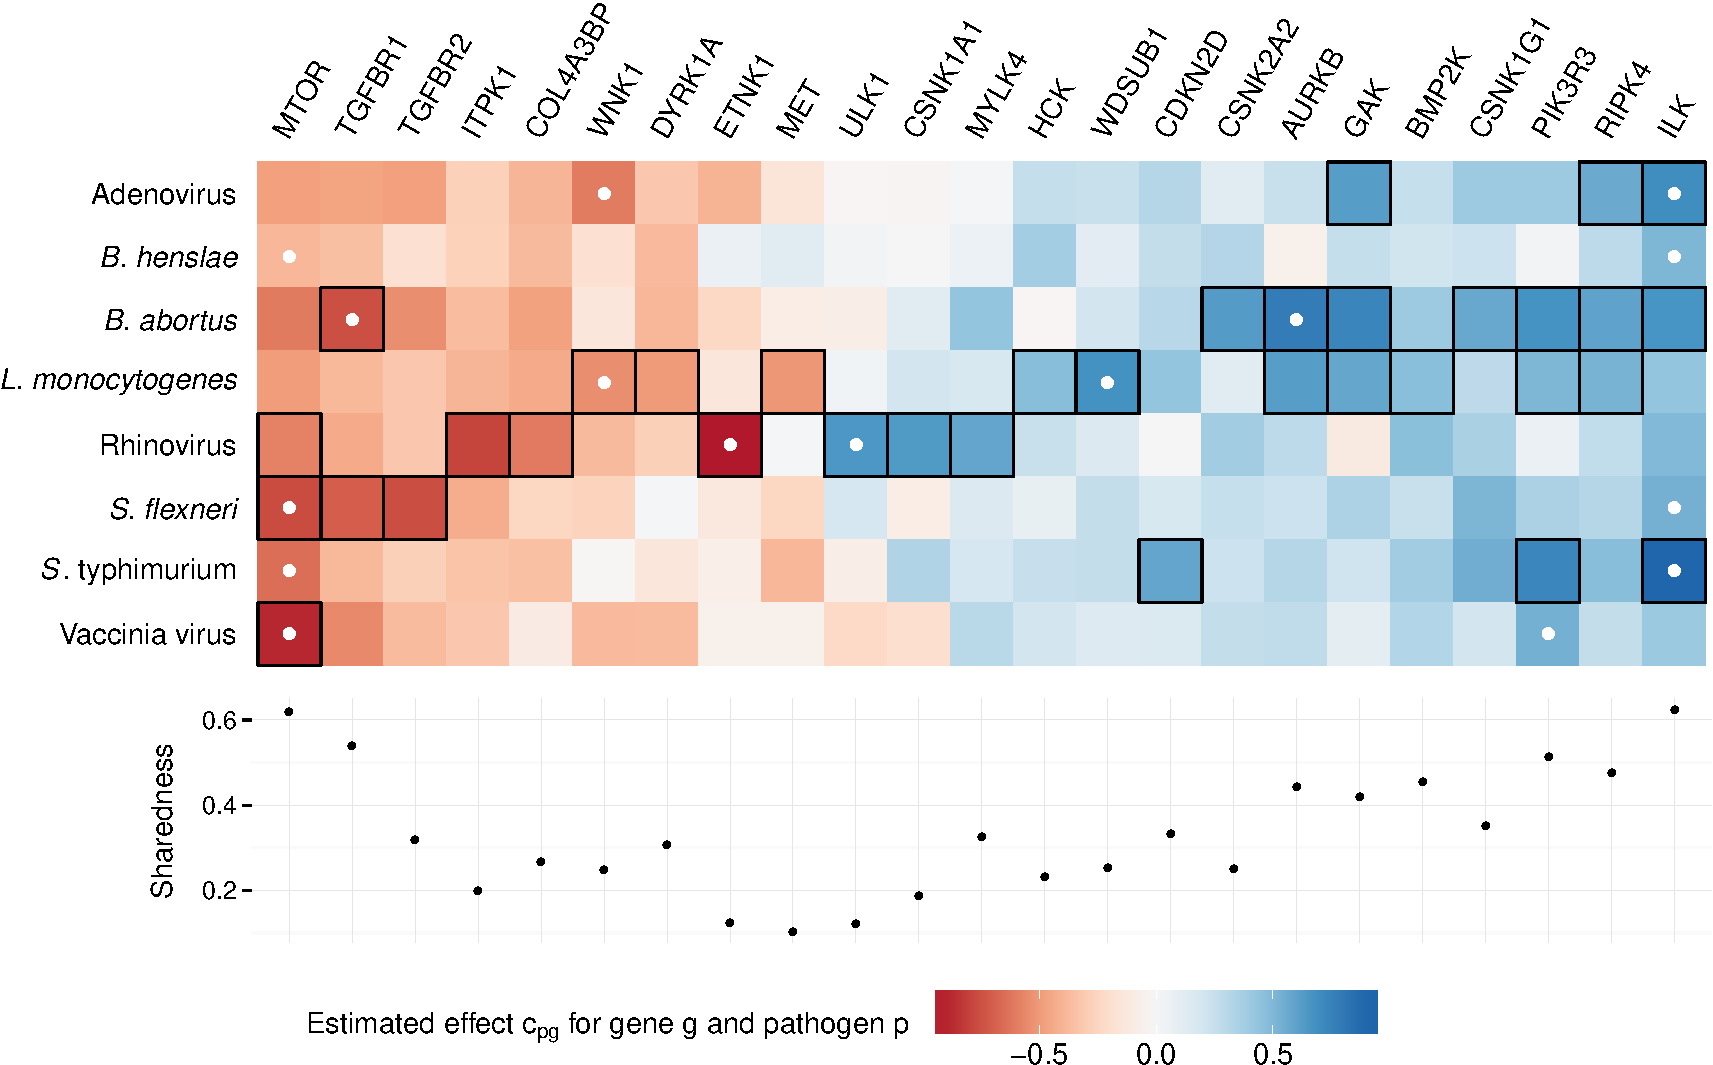
\includegraphics[width=.95\linewidth]{figures/R/pmm-pmm-heatmap-1} 

}

\caption[Heatmap plot showing significant genes for InfectX kinome screens as determined by pmm.]{A heatmap plot as produced by the Bioconductor package pmm, which displays all genes that were determined to be significant hits (FDR < 4; indicated by black borders) for at least one pathogen. Genes are ordered by average c\textunderscript{pg} values and both extrema are marked with white dots, while the sharedness score is shown as a scatterplot below. All available kinome screens were taken into consideration.}\label{fig:pmm-heatmap}
\end{figure}


\end{knitrout}




\begin{equation}
  \fdr(c_{pg}) = q_{pg} = \frac{\pi_0 f_0(c_{pg})}{f(c_{pg})}
\end{equation}

and represents the probability that the effect for a given gene and pathogen is a false discovery. Figure \ref{fig:pmm-heatmap} displays a visualization obtained by applying the PMM package (available on Bioconductor) to kinome-wide InfectX screens. Color-coding corresponds to estimated $c_{pg}$ effects and columns are sorted according to descending mean values. Only genes are included where the estimated \gls{fdr} is below 0.4 for at least one pathogen (indicated by black borders), suggesting that up to 40\% of individual hits may be superfluous. Centered white dots indicate the maximum and minimum $c_{pg}$ value for each pathogen. For each gene, a sharedness score is displayed as well. This quantity is defined as

\begin{equation}
  s_g = \frac{1}{2} \left(\left(1-\frac{1}{P}\sum_{p=1}^P q_{pg}\right) + \frac{\sum_{p=1}^P \mathds{1}_{q_{pg} < 1}}{P}\right)
\end{equation}

and quantifies how common a hit gene is among pathogens by describing both the extent of downward shift from 1 of the mean $q_{pg}$ value (over all $P=8$ pathogens), as well as the fraction of pathogens that contribute $q_{pg} < 1$ instances.

\section{Preliminary Findings}
Due to the high degree of redundancy in feature extraction during image analysis, a significant amount of correlation among features can be expected. Measurements of objects describing similar image segments, as well as features that build on related concepts, such as mean, median or integrated intensities, will obviously yield similar values and cause a dependence structure that has to be dealt with in statistical analysis. Figure \ref{fig:analysis-correlation} visualizes the issue by showing a heatmap representation of a correlation matrix, obtained from all available \textit{AreaShape}, \textit{Intensity} and \textit{Texture} features for a \textit{Brucella} plate using Dharmacon \gls{sirna} (J110-2D) and a randomly sampled subpopulation of cells (10\%).

The three feature groups can easily be spotted as diagonal blocks with high within group and lower between group correlation, and the situation is worst for intensity features due to the extensive set of measurements quantifying similar properties (see figure \ref{fig:intensity-features}). The texture segment is subdivided into four groups, corresponding from bottom left to top right to \textit{Cells}, \textit{Nuclei}, \textit{PeriNuclei} and \textit{VoronoiCells}. Absent off-diagonal correlation between nuclear and perinuclear regions is due to mutual exclusivity, whereas the off-diagonal correlation of cell and Voronoi cell features is due to significant overlap.

\begin{knitrout}
\definecolor{shadecolor}{rgb}{0.969, 0.969, 0.969}\color{fgcolor}\begin{figure}

{\centering 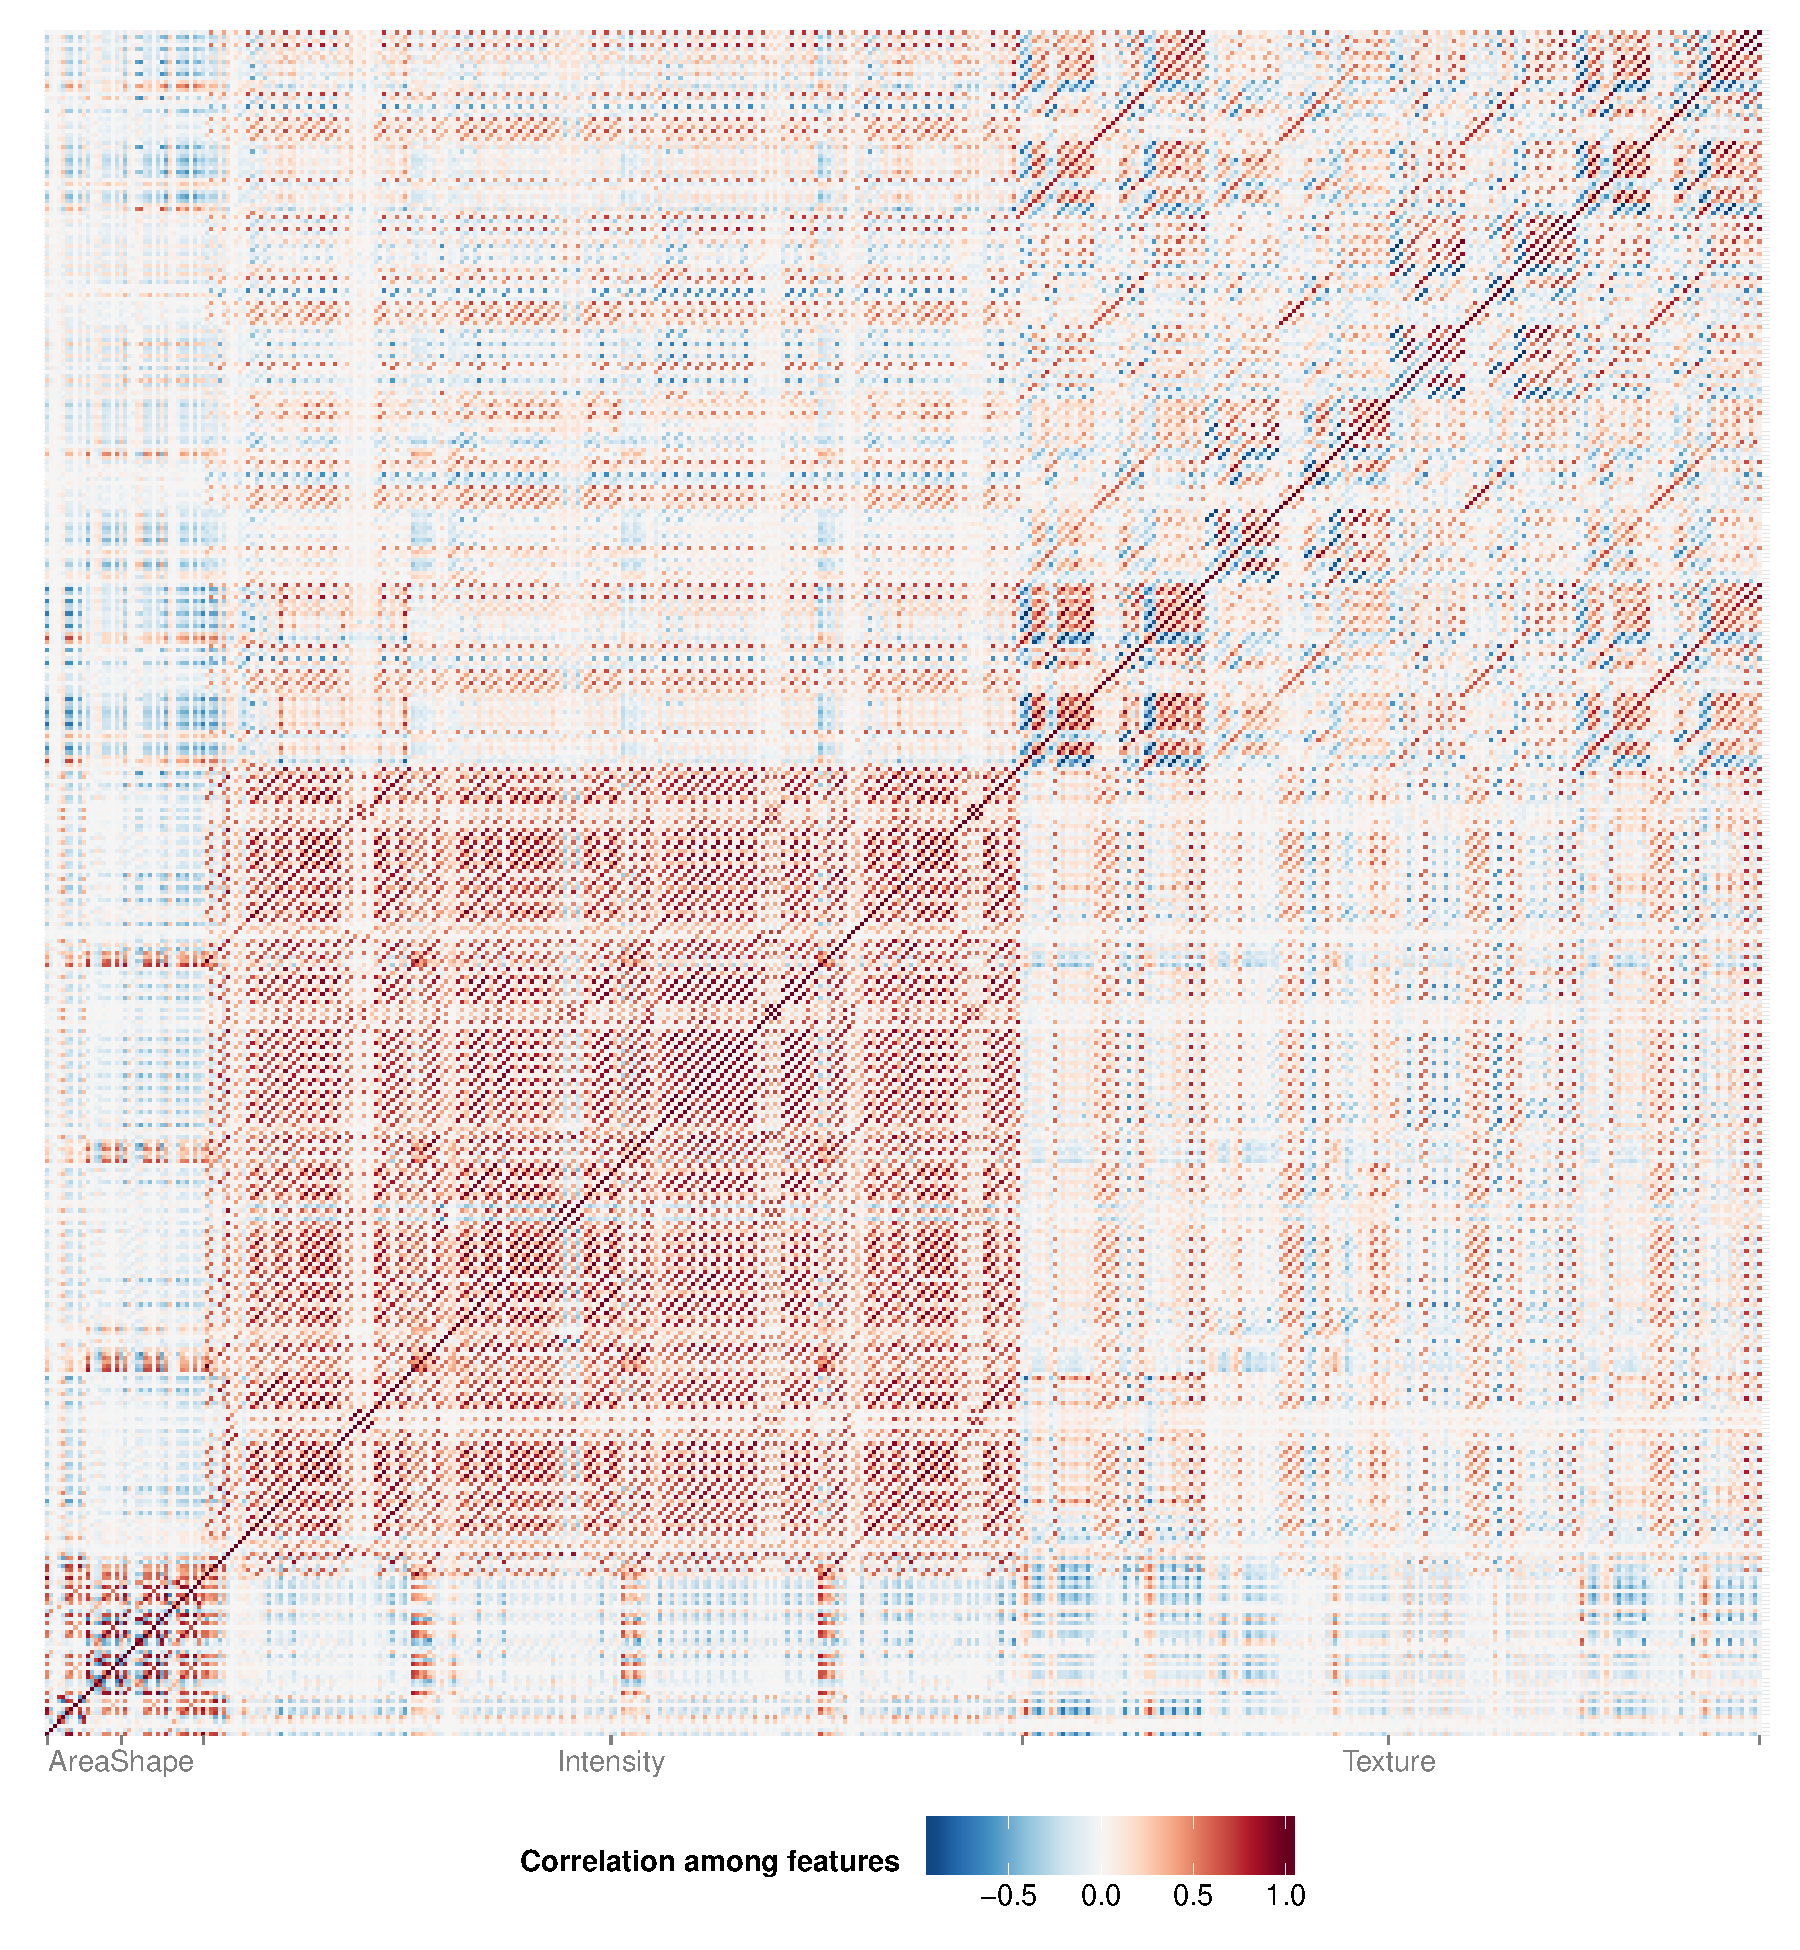
\includegraphics[width=\maxwidth]{figures/R/correlation-heatmap-analysis-correlation-1} 

}

\caption[Heatmap representation of correlation among single cell features.]{A heatmap representation of the correlation matrix obtained by sampling 10\% of single cell feature data available for plate J110-2D illustrates severe correlation among many features that is typical for all datasets. This comes as no surprise due to the redundancy in measured features. The three diagonal blocks correspond to three groups of features, \textit{AreaShape}, \textit{Intensity} and \textit{Texture}.}\label{fig:analysis-correlation}
\end{figure}


\end{knitrout}



In order to deal with this data issue, features are transformed to the coordinate system of \glspl{pc} prior to \gls{glm} model fitting. When employing \gls{pca}, typically the first 10\% of \glspl{pc} capture around 90\% of the overall variance in the data, corroborating the above claim of significant correlation among feature vectors. A further problem that is present in many datasets is that pairs of wells can be perfectly separated. This causes problems in maximum likelihood estimation, as affected coefficients are allowed to grow arbitrarily large, but is not unexpected given the large design space. \Gls{pca} provides a tool for addressing the issue by encouraging only inclusion of a subset of \glspl{pc} and thus reducing dimensionality.

Several \gls{glm} model fits, based on principal component regression are summarized in table \ref{tab:glm-1}. For the same plate is used in figure \ref{fig:analysis-correlation} (J110-2D, \textit{Brucella}, Dharmacon unpooled, replicate 1), well pairs corresponding to the genes identified by \gls{pmm} as down-hits, MTOR (H6) and PIK3R3 (K8), as well as up-hits, RIPK4 (G17) and TGFBR1 (M4), with respect to infection, are formed with all available scrambled wells of the given plate. In order to establish a baseline of sorts, scrambled wells are also paired with each other.

For describing how well the discrepancy between the two input wells is captured, some model characteristics, alongside scores for out-of-sample predictions are reported. The AIC is a goodness of fit estimate, constituting of the maximized log-likelihood $l$, as well as a penalty term for model size $k$, and is defined as

\begin{equation}
  \aic = 2k - 2l(\Hpi; y).
\end{equation}

Deviance values require caution when interpreted as a goodness-of-fit criterion, especially when used as an absolute measure, rather than being employed in a comparative capacity for nested models (analysis of deviance). The glm function of the R stats package reports both null deviance, defined as

\begin{equation}
  D^{(0)}(y; \pi^{(0)}) = 2l(\widetilde{\pi}; y) - 2l(\pi^{(0)}; y),
\end{equation}

with $\widetilde{\pi}$ denoting the saturated model, and residual deviance

\begin{equation}
  D(y; \Hpi) = 2l(\widetilde{\pi}; y) - 2l(\Hpi; y).
\end{equation}

The saturated model contains as many parameters as there are data observations ($n$) and consequently represents the maximally possible likelihood. The null model $\pi^{(0)}$ contains only an intercept term (i.e. a single parameter), while the proposed model $\Hpi$ attempts to explain the data using $p+1$ parameters (one for each covariate and an intercept). Finally, the values reported in table \ref{tab:glm-1} as $\Delta\textsubscript{deviance}$ are obtained as

\begin{equation}
  \Delta\textsubscript{deviance} = D^{(0)}(y; \pi^{(0)}) - D(y; \Hpi),
\end{equation}

therefore describing the difference between the quality of fit of the null model to that of the estimated model. Similarly, for the degrees of freedom, 

\begin{equation}
  \Delta\textsubscript{df} = \text{df}_\text{null} - \text{df}_\text{res} = n-1 -(n-(p+1)) = p.
\end{equation}

Under certain assumptions,\footnote{Deviance is only distributed as $\chi^2$ in the limit where for each $i \in \{1, 2, \dotsc, n\}$, the number of identical covariate rows $x_i$ grows to infinity. For continuous regressors, this is typically not the case, as the number of unique $x_i$ will often be very close to $n$. In case of binomially distributed response, the possibility of over-dispersion causes additional issues, which are not further described, as this does not apply to the current situation. Nevertheless, \citeauthor{Nelder1972} state that ``[t]he $\chi^2$ approximation is usually quite accurate for differences of deviances even though it is inaccurate for the deviances themselves.''} $\Delta\textsubscript{deviance} \mathbin{\sim} \chi^2_p$, and therefore a p-value for the significance of the model fit can be calculated. This is not reproduced, as all fits provide highly significant evidence against the null hypothesis, which assumes the fitted model to be no better than the null model.

\renewcommand{\arraystretch}{1.5}
\setlength{\tabcolsep}{0.25em}
\begin{table}
  \centering
  \caption[\Gls{glm} model summaries based on principal components for several well pairings.]{Summaries of several \gls{glm} models obtained by pairing wells corresponding to the genes MTOR (H6), PIK3R3 (K8), RIPK4 (G17) and TGFBR1 (M4) with all available scrambled wells on the same plate (J110-2D). Comparisons among scrambled wells serve as baseline (the scrambled row corresponds to well G1). Model fit is summarized by \gls{aic}, the difference in deviance and degrees of freedom (both between null and fitted models), as well as out-of-sample prediction scores. The following models suffer from separated data: MTOR (A24, G1, J2), PIK3R3 (E24, G1, G23, H2, L23), RIPK4 (E2, G23, H2, J2, L1) and Scrambled (A24, G23, H24, J24, L23).}
  \label{tab:glm-1}
  \footnotesize
  \begin{tabular}{llcccccccccccc}

 &  & A2 & A24 & E2 & E24 & G1 & G23 & H2 & H24 & J2 & J24 & L1 & \multicolumn{1}{c}{L23} \\ 
\hline
\nopagebreak MTOR & \nopagebreak AIC  & \multicolumn{1}{r}{1492} & \multicolumn{1}{r}{3251} & \multicolumn{1}{r}{1601} & \multicolumn{1}{r}{3140} & \multicolumn{1}{r}{1406} & \multicolumn{1}{r}{3541} & \multicolumn{1}{r}{1578} & \multicolumn{1}{r}{3139} & \multicolumn{1}{r}{1484} & \multicolumn{1}{r}{3213} & \multicolumn{1}{r}{1698} & \multicolumn{1}{r}{3781} \\
 & \nopagebreak \textDelta\textsubscript{deviance}  & \multicolumn{1}{r}{3343} & \multicolumn{1}{r}{1734} & \multicolumn{1}{r}{3205} & \multicolumn{1}{r}{2249} & \multicolumn{1}{r}{3552} & \multicolumn{1}{r}{1431} & \multicolumn{1}{r}{2785} & \multicolumn{1}{r}{1756} & \multicolumn{1}{r}{3436} & \multicolumn{1}{r}{1562} & \multicolumn{1}{r}{3152} & \multicolumn{1}{r}{1377} \\
 & \nopagebreak \textDelta\textsubscript{df}  & \multicolumn{1}{r}{46} & \multicolumn{1}{r}{48} & \multicolumn{1}{r}{48} & \multicolumn{1}{r}{47} & \multicolumn{1}{r}{46} & \multicolumn{1}{r}{48} & \multicolumn{1}{r}{48} & \multicolumn{1}{r}{48} & \multicolumn{1}{r}{48} & \multicolumn{1}{r}{48} & \multicolumn{1}{r}{47} & \multicolumn{1}{r}{48} \\
 & \rule{0pt}{1.7\normalbaselineskip}Accuracy  & \multicolumn{1}{r}{0.93} & \multicolumn{1}{r}{0.78} & \multicolumn{1}{r}{0.91} & \multicolumn{1}{r}{0.79} & \multicolumn{1}{r}{0.91} & \multicolumn{1}{r}{0.75} & \multicolumn{1}{r}{0.9} & \multicolumn{1}{r}{0.78} & \multicolumn{1}{r}{0.93} & \multicolumn{1}{r}{0.78} & \multicolumn{1}{r}{0.89} & \multicolumn{1}{r}{0.78} \\
 & \nopagebreak MCC  & \multicolumn{1}{r}{0.86} & \multicolumn{1}{r}{0.55} & \multicolumn{1}{r}{0.82} & \multicolumn{1}{r}{0.56} & \multicolumn{1}{r}{0.83} & \multicolumn{1}{r}{0.49} & \multicolumn{1}{r}{0.8} & \multicolumn{1}{r}{0.55} & \multicolumn{1}{r}{0.86} & \multicolumn{1}{r}{0.56} & \multicolumn{1}{r}{0.78} & \multicolumn{1}{r}{0.56} \\
\rule{0pt}{1.7\normalbaselineskip}PIK3R3 & \nopagebreak AIC  & \multicolumn{1}{r}{4471} & \multicolumn{1}{r}{4280} & \multicolumn{1}{r}{4075} & \multicolumn{1}{r}{4954} & \multicolumn{1}{r}{3509} & \multicolumn{1}{r}{3742} & \multicolumn{1}{r}{3401} & \multicolumn{1}{r}{4396} & \multicolumn{1}{r}{3779} & \multicolumn{1}{r}{3212} & \multicolumn{1}{r}{4170} & \multicolumn{1}{r}{3214} \\
 & \nopagebreak \textDelta\textsubscript{deviance}  & \multicolumn{1}{r}{882} & \multicolumn{1}{r}{1245} & \multicolumn{1}{r}{1244} & \multicolumn{1}{r}{1044} & \multicolumn{1}{r}{1990} & \multicolumn{1}{r}{1769} & \multicolumn{1}{r}{1404} & \multicolumn{1}{r}{1025} & \multicolumn{1}{r}{1672} & \multicolumn{1}{r}{2068} & \multicolumn{1}{r}{1200} & \multicolumn{1}{r}{2512} \\
 & \nopagebreak \textDelta\textsubscript{df}  & \multicolumn{1}{r}{48} & \multicolumn{1}{r}{49} & \multicolumn{1}{r}{50} & \multicolumn{1}{r}{49} & \multicolumn{1}{r}{49} & \multicolumn{1}{r}{49} & \multicolumn{1}{r}{49} & \multicolumn{1}{r}{49} & \multicolumn{1}{r}{50} & \multicolumn{1}{r}{49} & \multicolumn{1}{r}{49} & \multicolumn{1}{r}{49} \\
 & \rule{0pt}{1.7\normalbaselineskip}Accuracy  & \multicolumn{1}{r}{0.71} & \multicolumn{1}{r}{0.71} & \multicolumn{1}{r}{0.76} & \multicolumn{1}{r}{0.69} & \multicolumn{1}{r}{0.77} & \multicolumn{1}{r}{0.8} & \multicolumn{1}{r}{0.74} & \multicolumn{1}{r}{0.75} & \multicolumn{1}{r}{0.77} & \multicolumn{1}{r}{0.81} & \multicolumn{1}{r}{0.7} & \multicolumn{1}{r}{0.84} \\
 & \nopagebreak MCC  & \multicolumn{1}{r}{0.41} & \multicolumn{1}{r}{0.42} & \multicolumn{1}{r}{0.51} & \multicolumn{1}{r}{0.38} & \multicolumn{1}{r}{0.54} & \multicolumn{1}{r}{0.6} & \multicolumn{1}{r}{0.47} & \multicolumn{1}{r}{0.49} & \multicolumn{1}{r}{0.55} & \multicolumn{1}{r}{0.63} & \multicolumn{1}{r}{0.4} & \multicolumn{1}{r}{0.67} \\
\rule{0pt}{1.7\normalbaselineskip}RIPK4 & \nopagebreak AIC  & \multicolumn{1}{r}{4064} & \multicolumn{1}{r}{5554} & \multicolumn{1}{r}{3596} & \multicolumn{1}{r}{6047} & \multicolumn{1}{r}{3076} & \multicolumn{1}{r}{4918} & \multicolumn{1}{r}{3161} & \multicolumn{1}{r}{5055} & \multicolumn{1}{r}{3366} & \multicolumn{1}{r}{4580} & \multicolumn{1}{r}{4094} & \multicolumn{1}{r}{4731} \\
 & \nopagebreak \textDelta\textsubscript{deviance}  & \multicolumn{1}{r}{1751} & \multicolumn{1}{r}{455} & \multicolumn{1}{r}{2179} & \multicolumn{1}{r}{498} & \multicolumn{1}{r}{2900} & \multicolumn{1}{r}{1075} & \multicolumn{1}{r}{2037} & \multicolumn{1}{r}{837} & \multicolumn{1}{r}{2560} & \multicolumn{1}{r}{1153} & \multicolumn{1}{r}{1740} & \multicolumn{1}{r}{1506} \\
 & \nopagebreak \textDelta\textsubscript{df}  & \multicolumn{1}{r}{48} & \multicolumn{1}{r}{49} & \multicolumn{1}{r}{49} & \multicolumn{1}{r}{49} & \multicolumn{1}{r}{48} & \multicolumn{1}{r}{49} & \multicolumn{1}{r}{49} & \multicolumn{1}{r}{49} & \multicolumn{1}{r}{50} & \multicolumn{1}{r}{49} & \multicolumn{1}{r}{49} & \multicolumn{1}{r}{49} \\
 & \rule{0pt}{1.7\normalbaselineskip}Accuracy  & \multicolumn{1}{r}{0.81} & \multicolumn{1}{r}{0.65} & \multicolumn{1}{r}{0.81} & \multicolumn{1}{r}{0.61} & \multicolumn{1}{r}{0.85} & \multicolumn{1}{r}{0.72} & \multicolumn{1}{r}{0.82} & \multicolumn{1}{r}{0.64} & \multicolumn{1}{r}{0.84} & \multicolumn{1}{r}{0.71} & \multicolumn{1}{r}{0.79} & \multicolumn{1}{r}{0.74} \\
 & \nopagebreak MCC  & \multicolumn{1}{r}{0.61} & \multicolumn{1}{r}{0.29} & \multicolumn{1}{r}{0.61} & \multicolumn{1}{r}{0.22} & \multicolumn{1}{r}{0.7} & \multicolumn{1}{r}{0.44} & \multicolumn{1}{r}{0.62} & \multicolumn{1}{r}{0.27} & \multicolumn{1}{r}{0.67} & \multicolumn{1}{r}{0.42} & \multicolumn{1}{r}{0.57} & \multicolumn{1}{r}{0.48} \\
\rule{0pt}{1.7\normalbaselineskip}Scrambled & \nopagebreak AIC  & \multicolumn{1}{r}{4673} & \multicolumn{1}{r}{2480} & \multicolumn{1}{r}{4366} & \multicolumn{1}{r}{2843} & \multicolumn{1}{c}{--} & \multicolumn{1}{r}{2130} & \multicolumn{1}{r}{3731} & \multicolumn{1}{r}{2800} & \multicolumn{1}{r}{4673} & \multicolumn{1}{r}{1651} & \multicolumn{1}{r}{4670} & \multicolumn{1}{r}{1885} \\
 & \nopagebreak \textDelta\textsubscript{deviance}  & \multicolumn{1}{r}{670} & \multicolumn{1}{r}{3032} & \multicolumn{1}{r}{941} & \multicolumn{1}{r}{3140} & \multicolumn{1}{c}{--} & \multicolumn{1}{r}{3368} & \multicolumn{1}{r}{1065} & \multicolumn{1}{r}{2610} & \multicolumn{1}{r}{765} & \multicolumn{1}{r}{3615} & \multicolumn{1}{r}{687} & \multicolumn{1}{r}{3827} \\
 & \nopagebreak \textDelta\textsubscript{df}  & \multicolumn{1}{r}{48} & \multicolumn{1}{r}{48} & \multicolumn{1}{r}{49} & \multicolumn{1}{r}{48} & \multicolumn{1}{c}{--} & \multicolumn{1}{r}{48} & \multicolumn{1}{r}{49} & \multicolumn{1}{r}{49} & \multicolumn{1}{r}{49} & \multicolumn{1}{r}{47} & \multicolumn{1}{r}{48} & \multicolumn{1}{r}{48} \\
 & \rule{0pt}{1.7\normalbaselineskip}Accuracy  & \multicolumn{1}{r}{0.69} & \multicolumn{1}{r}{0.89} & \multicolumn{1}{r}{0.69} & \multicolumn{1}{r}{0.86} & \multicolumn{1}{c}{--} & \multicolumn{1}{r}{0.88} & \multicolumn{1}{r}{0.74} & \multicolumn{1}{r}{0.85} & \multicolumn{1}{r}{0.7} & \multicolumn{1}{r}{0.92} & \multicolumn{1}{r}{0.65} & \multicolumn{1}{r}{0.9} \\
 & \nopagebreak MCC  & \multicolumn{1}{r}{0.38} & \multicolumn{1}{r}{0.77} & \multicolumn{1}{r}{0.39} & \multicolumn{1}{r}{0.73} & \multicolumn{1}{c}{--} & \multicolumn{1}{r}{0.76} & \multicolumn{1}{r}{0.46} & \multicolumn{1}{r}{0.7} & \multicolumn{1}{r}{0.4} & \multicolumn{1}{r}{0.83} & \multicolumn{1}{r}{0.31} & \multicolumn{1}{r}{0.81} \\
\rule{0pt}{1.7\normalbaselineskip}TGFBR1 & \nopagebreak AIC  & \multicolumn{1}{r}{3897} & \multicolumn{1}{r}{4968} & \multicolumn{1}{r}{3807} & \multicolumn{1}{r}{5529} & \multicolumn{1}{r}{3683} & \multicolumn{1}{r}{4825} & \multicolumn{1}{r}{3244} & \multicolumn{1}{r}{4969} & \multicolumn{1}{r}{3589} & \multicolumn{1}{r}{3887} & \multicolumn{1}{r}{4335} & \multicolumn{1}{r}{4722} \\
 & \nopagebreak \textDelta\textsubscript{deviance}  & \multicolumn{1}{r}{2018} & \multicolumn{1}{r}{1147} & \multicolumn{1}{r}{2069} & \multicolumn{1}{r}{1135} & \multicolumn{1}{r}{2400} & \multicolumn{1}{r}{1273} & \multicolumn{1}{r}{2040} & \multicolumn{1}{r}{1025} & \multicolumn{1}{r}{2439} & \multicolumn{1}{r}{1944} & \multicolumn{1}{r}{1599} & \multicolumn{1}{r}{1626} \\
 & \nopagebreak \textDelta\textsubscript{df}  & \multicolumn{1}{r}{47} & \multicolumn{1}{r}{48} & \multicolumn{1}{r}{49} & \multicolumn{1}{r}{48} & \multicolumn{1}{r}{48} & \multicolumn{1}{r}{48} & \multicolumn{1}{r}{49} & \multicolumn{1}{r}{48} & \multicolumn{1}{r}{49} & \multicolumn{1}{r}{48} & \multicolumn{1}{r}{48} & \multicolumn{1}{r}{48} \\
 & \rule{0pt}{1.7\normalbaselineskip}Accuracy  & \multicolumn{1}{r}{0.81} & \multicolumn{1}{r}{0.71} & \multicolumn{1}{r}{0.8} & \multicolumn{1}{r}{0.69} & \multicolumn{1}{r}{0.81} & \multicolumn{1}{r}{0.71} & \multicolumn{1}{r}{0.8} & \multicolumn{1}{r}{0.7} & \multicolumn{1}{r}{0.85} & \multicolumn{1}{r}{0.8} & \multicolumn{1}{r}{0.77} & \multicolumn{1}{r}{0.77} \\
 & \nopagebreak MCC  & \multicolumn{1}{r}{0.6} & \multicolumn{1}{r}{0.41} & \multicolumn{1}{r}{0.6} & \multicolumn{1}{r}{0.39} & \multicolumn{1}{r}{0.62} & \multicolumn{1}{r}{0.42} & \multicolumn{1}{r}{0.57} & \multicolumn{1}{r}{0.38} & \multicolumn{1}{r}{0.69} & \multicolumn{1}{r}{0.59} & \multicolumn{1}{r}{0.53} & \multicolumn{1}{r}{0.53} \\
\hline 
\end{tabular}


%\newcommand{\knitrDataGlm1PerSepScram}{pasteAnd(names(perfect.sep$Scrambled)[which(perfect.sep$Scrambled)])}
%\newcommand{\knitrDataGlm1PerSepMtor}{pasteAnd(names(perfect.sep$MTOR)[which(perfect.sep$MTOR)])}
%\newcommand{\knitrDataGlm1PerSepTgfbr1}{pasteAnd(names(perfect.sep$TGFBR1)[which(perfect.sep$TGFBR1)])}
%\newcommand{\knitrDataGlm1PerSepRipk4}{pasteAnd(names(perfect.sep$RIPK4)[which(perfect.sep$RIPK4)])}
%\newcommand{\knitrDataGlm1PerSepPik3r3}{pasteAnd(names(perfect.sep$PIK3R3)[which(perfect.sep$PIK3R3)])}

\end{table}

Moving along to out-of-sample prediction scores, table \ref{tab:glm-1} shows both accuracy and \gls{mcc} values obtained by separating 20\% of data for each group from training data and evaluating predictions. Accuracy is defined as

\begin{equation}
  \text{Acc} = \frac{n_{tp} + n_{tn}}{n_p+n_n}
\end{equation}

where $n_{tp}$ represents the number of true positives, $n_{tn}$ the count of true negatives and $p$, $n$ the number of positive and negative instances, respectively. The \acrshort{mcc} \citep{Matthews1975} can be evaluated as

\begin{equation}
  \text{Mcc} = \frac{n_{tp} n_{tn} - n_{fp} n_{fn}}{\sqrt{(n_{tp} + n_{fp})(n_{tp} + n_{fn})(n_{tn} + n_{fp})(n_{tn} + n_{fn})}}
\end{equation}

and $n_{fp}$, $n_{fn}$ correspond to false positives and false negatives. Values for \gls{mcc} range from $-1$ (total disagreement) to $1$ (perfect prediction), and the midpoint $0$ indicates random prediction.

Given these model characteristics, two patterns emerge: (1) the ability to distinguish two wells is dependent on well distance within the plate and (2) the differences among scrambled wells, in terms of computed quality of fit estimates, are comparable to those that are observed when modeling the discrepancy between hit genes and control wells. To make the first claim, well locations are required: MTOR (H6), PIK3R3 (K8), RIPK4 (G17), TGFBR1 (M4) and Scrambled (A2, A24, E2, E24, G1, G23, H2, H24, J2, J24, L1 and L23). For both MTOR and TGFBR1, which represent early-row, down-hit genes, an alternating sequence is clearly discernible and is characterized by lower AIC, larger $\Delta\textsubscript{deviance}$ and better predictive power for wells that are closer together, while the opposite holds for comparisons among scrambled wells. The effect is less distinct for PIK3R3 and RIPK4 which both are located more towards the plate center and are identified as up-hits. For RIPK4 the alternations are still noticeable albeit, as in scrambled, polarity is reversed. This is indicative of some technical artifacts contained in the data, that dominate biological features of interest. Furthermore, the excellent predictions that can be made based on membership to either one of a scrambled well pair is disconcerting, as biologically they should be equivalent. Again, technical effects seemingly dominate.

In 18 of the 59 models displayed in table \ref{tab:glm-1}, a warning regarding perfectly separated data is issued by the glm routine (in the example of MTOR, wells A24, G1 and J2). For this particular case, the matter is not further investigated, as it does not have obviously relevant consequences.\footnote{For other inquiries, not reported here, perfect separation was addressed by reducing the number of \glspl{pc} or using regularized procedures. Furthermore the issue was studied by solving associated linear programming problems in order to explicitly find the separating hyperplane and thus determine whether this is actually part of the data or caused by numerical shortcomings of the glm implementation. In an example by \citeauthor{Gelman2015} it is shown that a response such as \mintinline{text}{y <- rep (c(1,0),c(10,5))} in a model containing only an intercept, will trigger the separation warning dependent on starting values (i.e. using \mintinline{text}{start=2.6}, glm runs fine, whereas \mintinline{text}{start=2.7} issues the warning). A further effect known to cause problems under certain circumstances, especially for convergence, is the Hauck-Donner phenomenon. As it turns out, separating hyperplanes can reliably be determined, most probably owing in part to the high dimensional setting.} Affected data points appear in line with well pairs where no complete data separation is possible and the above arguments still hold if possibly questionable data is excluded (albeit patterns are less clearly distinguishable).

Apart from the results shown, many similar investigations were performed, using other datasets and\slash or slightly different methods. Further \textit{Brucella} plates were considered, pooled \gls{sirna} experiments, libraries from Ambion and Qiagen, as were several \textit{Salmonella} plates and for some inquiries, cell population was limited to infected only. Method-wise, ridge and elastic net penalized regression (glmnet), other glm implementations, such as glm2 (\cite{Marschner2014}; uses a more robust fitting procedure), brglm (\cite{Kosmidis2013}; deals with data separation by penalized maximum likelihood) and bayesglm (\cite{Gelman2015}; regularizes coefficients though a weakly informative prior distribution), as well as step-wise model building (using the step function of the R stats package) was explored.

% bootstrapped stuff

All analysis performed clearly indicates that for the intended type of modeling, an effective normalization scheme has to be developed that is able to capture technical effects (and perhaps even spurious biological artifacts), without destroying phenotypic information coming from gene knockdown and pathogen infection. Attempts of achieving this are outlined in the following section.

\section{Data Normalization}
The large amount of technical variation, coupled with treating biological systems, which in turn are associated with their own inherent noise, make the analysis of \gls{hts} data a challenging endeavor, requiring thorough normalization procedures. The poor reproducibility that often plagues \gls{sirna} experiments may be addressed and even resolved with the availability of effective corrections that do not negatively affect phenotypes of interest. The following sections outline two types of normalization approaches, plate and well level corrections via Z-scoring\slash B-scoring and using residuals of a \gls{mars} model at a single cell level, as well as their effect on InfectX datasets.

\subsection{Plate and Well Level Normalization}
In order to correct \gls{sirna} data for experimental artifacts at plate and well levels, two schemes have become standard practice, Z-scoring and B-scoring \citep{Malo2006}. The former is widely known (outside the field of \gls{sirna} analysis) and is defined as

\begin{equation}
  z_i = \frac{x_i - \mu}{\sigma}
\end{equation}

where $\mu$ represents the mean, $\sigma$ the standard deviation and $x$ the vector of features to be normalized. Applying Z-scoring both centers data around zero and scales variability to unit variance. B-scoring is more domain specific and deals with row and column effects that have been discussed previously (e.g. pipetting issues, leading to horizontal patterns or temporal effects such as decay of actin stain intensity, resulting in a vertically oriented gradient, when imaging is performed column-wise). B-scoring can be expressed as

\begin{equation}
  b_{ijp} = \frac{r_{ijp}}{\mad(r)} = \frac{x_{ijp} - (\Hmu_p + \widehat{\alpha}_{ip} + \widehat{\beta}_{jp})}{\mad(r)}
\end{equation}

and estimates for row and column effects, $\widehat{\alpha}_{ip}$ and $\widehat{\beta}_{jp}$, respectively, are obtained by fitting a two-way median polish algorithm. Together with an estimate for plate average $\Hmu_p$, these three parameters are used to determine a residual $r_{ijp}$, which divided by the \gls{mad} over the whole plate, yields the B-scored value $b_{ijp}$. Median polishing proceeds by augmenting the plate layout with an additional column and row as

\begin{equation*}
  \begin{array}{cccc|c}
    r_{1,1,p} & r_{1,2,p} & \cdots & r_{1,24,p} & \alpha_{1,p} \\
    r_{2,1,p} & r_{2,2,p} & \cdots & r_{2,24,p} & \alpha_{2,p} \\
    \vdots  & \vdots  & \ddots & \vdots & \vdots \\
    r_{16,1,p} & r_{16,2,p} & \cdots & r_{16,24,p} & \alpha_{16,p} \\
    \hline
    \beta_{1,p} & \beta_{2,p} & \cdots & \beta_{24,p} & \mu_{p} \\
  \end{array}
\end{equation*}

and initializing the values as $r_{ijp} = x_{ijp}$ and $\alpha_{i,p} = \beta_{j,p} = \mu_p = 0$. A row sweep consists of iterating all rows, calculating the median of $(r_{i,1,p}, r_{i,2,p}, \dotsc, r_{i,24,p})$ for each row $i$, subtracting the resulting value from $(r_{i,1,p}, r_{i,2,p}, \dotsc, r_{i,24,p})$ and adding it to $\alpha_{i,p}$. The same procedure is also applied to the column effect row where the median of $(\beta_{1,p}, \beta_{2,p}, \dotsc, \beta_{24,p}$ is subtracted from $(\beta_{1,p}, \beta_{2,p}, \dotsc, \beta_{24,p}$ and added to $\mu_p$). A column sweep is carried out analogously and the two procedures are alternated until all rows and columns of residuals have median zero, as do the vectors of row and column effects (or fall below a threshold close to zero). Usually only few pairs of sweeps ($\sim 2$) are needed and the results are non-unique as they depend on whether row or column sweeps are put first. Furthermore, using means instead of medians yields a least squares decomposition as in two-way \gls{anova} without iteration, which is less robust towards outliers \citep{Brown2004,Venables2002}. The \gls{mad} is defined as

\begin{equation}
  \mad(x) = \median\left(\abs{x_i-\median(x)}\right).
\end{equation}

and therefore provides a robust estimation of data spread which is more resilient towards outliers as other measures of dispersion, such as standard deviation.

While B-scoring has proven to be a capable normalization tool for data coming from a plate reader or phenotypic data like infection scores as generated from InfectX screens, where there is a single value per well to be adjusted for experimental artifacts, the situation for single cell feature data is much more complex. Ideally, Z-scoring and B-scoring are able to correct for concerns at plate and well level, but data hierarchy goes beyond that for InfectX datasets. First, data can be split into images which are captured individually, possibly with different imaging parameters and therefore may require differing treatment.

\subsection{\Acrlong{mars}}
At cellular level of granularity, an abundance of additional sources of noise may directly be addressed. This includes technical issues, as well as biological variability. Examples for the former include location of cell within well which might be relevant due some degree of curvature of the well bottom, inducing focusing problems towards well borders, or location of cell within image, possibly affecting cellular features due to varying optical properties moving away from the image center (e.g. vignetting, decrease in sharpness, chromatic aberration, etc.). Biological sources of noise are even more plentiful and therefore increasingly harder to address. Obvious targets are general cell state parameters, such as cell cycle stage or whether the cell is apoptotic with the difficulty here being reliably determining these factor variables.

Work by \citeauthor{Snijder2012} elucidates the importance of cellular population context in cell-to-cell variability. In a comprehensive analysis of virally perturbed \gls{sirna} screens they demonstrate that parameters such as local cell density, population size and cell location within cellular aggregates significantly alter measured phenotypes. Building on these results, \citeauthor{Knapp2011} devised a normalization scheme by fitting a \gls{mars} model to a selection of features that represent the cellular population context and using only the residuals for further analysis.

\Gls{mars} is an nonparametric regression procedure for finding a piecewise linear solution that makes no assumptions on data distributions and is highly capable in a high-dimensional setting with respect to predictor variables. The following short introduction into \gls{mars} modeling is largely based on \cite{Hastie2009}. Basis functions of the form

\begin{equation}
  (x_j-t)_+ = \max(0, x_j-t) =
  \begin{cases}
    x_j-t,& \text{if } x_j > t\\
    0,              & \text{otherwise},
  \end{cases}
\end{equation}

and $(t-x_j)_+$, which form reflected pairs, are used for describing the model surface. Such linear splines contain a knot at value $t$ which separates the function support into a zero part and a nonzero domain while for the reflected version the two regions are swapped with opposite slope. Despite each basis function only depending on a single covariate ($j \in \{1, 2, \dotsc, p\}$), they are still considered as functions over the complete predictor space $\R^p$. Model building proceeds by maintaining two sets of reflected pairs, candidates and active pairs, where the active set initially contains only a constant term and candidates include all $2np$ possible functions with knots at each observed value $x_{ij}$

\begin{equation}
  C = \left\{(x_j-t)_+, (t-x_j)_+ \given t\in\{x_{1j}, x_{2j}, \dotsc, x_{nj}, \} \land j\in\{1, 2, \dotsc, p\} \right\}.
\end{equation}

A \gls{mars} model has the form

\begin{equation}
  g(x) = \mu + \sum_{m=1}^M \beta_m h_m(x),
\end{equation}

where the coefficients $\beta_m$ represent slopes of basis functions $h_m(\cdot)$ which can either be chosen from individual functions in C or by forming products of functions from the set of candidates C and thereby directly model interactions between variables. The active set is initialized with $A=\{h_0(x)=1\}$ and in an iterative procedure, for $k=1, 2, \dotsc, M$, the best pair of functions $\{h_{2k-1}(x), h_{2k}(x)\}$ with respect to the largest reduction in residual sum of squares is chosen and added to the active set, whereby the new additions are products of a reflected pair from the candidate set with a function $h_l(x)$ of the active set

\begin{subequations}
\begin{align}
  h_{2k-1}(x) &= h_l(x) \cdot (x_j-t)_+ \\
  h_{2k}(x) &= h_l(x) \cdot (t-x_j)_+.
\end{align}
\end{subequations}

The $2k$ coefficients are estimated by least squares and in each step the model grows by two basis functions. The iteration process is terminated when a preset number of basis functions have been added to the active set, typically leading to a model that over-fits the data. A pruning scheme follows that from each pair of functions $\{h_{2k-1}(x), h_{2k}(x)\}$, removes the one that yields the smaller increase in residual sum of squares. In order to determine the right amount of backwards elimination and find the best model $\widehat{g}_\lambda^{\ *}(x)$, for each stage, a \gls{gcv} score is computed for the current model $\widehat{g}_\lambda(x)$. A further possibility is performing cross validation but this is often foregone due to computational expense. The \gls{gcv} criterion is defined as

\begin{equation}
  \text{gcv}(\lambda) = \frac{1}{n}\frac{\sum_{i=1}^n \left(y_i-\widehat{g}_\lambda(x_i)\right)^2}{\left(1-\frac{C(\lambda)}{n}\right)^2},
\end{equation}

where cost complexity term $C(\lambda)$ represents the effective number of parameters, computed as a sum of the number of linearly independent basis functions with the product of a smoothing parameter $d$ and the number of terms. The value of $d$ is typically 2 (additive model) or 3 (higher orders allowed) and controls the amount of kinks introduced \citep{Friedman1991}.

By having the option of combining functions in the active set with newly entering terms, the algorithm builds a hierarchical model in the sense that interactions of added variables are only possible if all interacting partners are already present, forming an interaction of one order less. The reasoning behind this is that otherwise the search space would grow exponentially, causing computational issues for higher order interactions and in many cases it seems justifiable to require main effects as basis for interactions. Furthermore, the formation of powers is not allowed as a term may only enter a single time in an iteration, again limiting the search space for computational efficiency. For interpretability and in larger problems for performance reasons, it is often advisable to restrict the number of interactions to degree 2 or 3.

\subsection{Normalization of Single Cell Data}
For normalization of InfectX data, two 

%\section{Modeling Approach}
\section{Outlook and Conclusion}